%% План книги
%% ТеХ для всех - издание третье, дополненное и существенно переработанное.

%% 9 августа 2013

%% Авторский коллектив:
%% Беляков Н.С.
%% Палош В.Е.
%% Садовский П.А.

% % Cм Разбивку глав по авторам!

\documentclass[a4paper,11pt]{book}



\usepackage[utf8]{inputenc}
\usepackage[T2A]{fontenc}
\usepackage[english, german, francais, russian]{babel}

\renewcommand\baselinestretch{0.92}

% Общее оформление: 
% Замечание и Внимание: вернуть значки...

% Выравнивание по середине...
% Цитаты - ОК
% красивая заглавная буква...



% Касательно стилевика или разметки - наверно, я бы переделал по аналогии с издательством Springer, очень уж у них читаемо и красиво... Ну и в целом - грамотно сделано. Шрифт можно слегка уменьшить, размер листа - увеличить (правда, нужно посмотреть другие книги изд-ва УРСС - что у них там есть в плане стандартных форматов).

%% Geometry of the Layout
%\usepackage[marginparsep=1mm, width=112mm, headsep=10pt, includehead, headheight=14pt, textheight=172mm, centering, twoside]{geometry}

\usepackage[dvips=false,pdftex=false,vtex=false]{geometry}% Формат 70x100/16
\geometry{
	paperwidth=175mm,
	paperheight=250mm,
	marginparsep=1mm,
	width=135mm, 
	headsep=10pt, 
	includehead, 
	headheight=14pt, 
	textheight=203mm, 
	centering, 
	twoside
}
\usepackage[cam,dvips,a4,center]{crop}
\crop[cam]

%\usepackage[marginparsep=1mm, width=117mm, headsep=10pt, includehead, headheight=14pt, textheight=185mm, centering, twoside]{geometry} % Формат 60x90/16



%   Общеупотребительные форматы книг              набор        после о. Наука п.о.  до обр.
% \DeclareOption{60x90/16}{\def\form@t{8}}  % 113-122*180-190  145*215  140*215     150*225
% \DeclareOption{70x90/16}{\def\form@t{9}}  % 135-144*180-190  170*215  164*215     175*225
% \DeclareOption{70x100/16}{\def\form@t{11}}% 135-144*199-208  170*240  164*235     175*250


% \textwidth=112mm \textheight=185mm % 60x90/16   113-122*180-190
% \textwidth=134mm \textheight=185mm % 70x90/16   135-144*180-190
% \textwidth=134mm \textheight=203mm % 70x100/16  135-144*199-208




%% For indents of the 1st line of paragraph after section name
\usepackage{indentfirst}

%% For Colors
%\usepackage{xcolor}
\usepackage[table]{xcolor}
%\usepackage{color}
\usepackage{colortbl}

%% For Lists
\usepackage{paralist}
\usepackage{enumerate}
%\usepackage{enumitem}


%% For Footnotes
\usepackage{footnote}
\usepackage{ctable}

% % For Chemistry
\usepackage[version=3]{mhchem}


%% For Tables
\usepackage{array}
\usepackage{multirow}
\usepackage{longtable}
%\usepackage{slashbox}
\usepackage{booktabs}
\usepackage[labelsep=period]{caption}
\usepackage{wrapfig}
\usepackage{sidecap}
\usepackage{subfig}
\usepackage{xtab}

%% For Maths
\usepackage{amsmath, amssymb}
\usepackage{mathtools}
\usepackage{amsthm}


%% For Multi-Column typing
\usepackage{multicol}


\usepackage{mflogo}

%\usepackage{tikz}

% % For Music
% %\usepackage{musixtex}


\usepackage{marvosym}
%\usepackage{tipa}



\usepackage{verbatim}
\usepackage[multiple]{footmisc}

% % Предметный указатель
% %\usepackage{showidx}
\usepackage{makeidx}		% для создания указателя
%\usepackage{index}
\makeindex


% Bold Italic
%\newcommand{\bi}[1]{\textbf{\textit{#1}}}

\makeatletter

\input{Definitions-1}

\let\bibfont=\small
\def\@biblabel#1{#1.}


\def\pkg#1{\bgroup\ttfamily#1\egroup}

% Добавляет команду с \ в индекс, но не выводит ее в тексте
\def\indcom#1{\index{#1@\comm{#1}}}

% Добавляет команду с \ в индекс и выводит ее в тексте
\def\indcmd#1{\index{#1@\comm{#1}}\comm{#1}}


% Добавляет пакет в индекс, но не выводит его в тексте
\def\indpak#1{\index{#1@\pkg{#1}}}

% добавляет пакет в индекс и выводит в тексте
\def\indpkg#1{\index{#1@\pkg{#1}}\pkg{#1}}





%\newcommand{\comm}[1]{\bgroup\ttfamily\textbackslash#1\egroup}
%\newcommand{\ltfamily}{\fontfamily{tli}\selectfont}
%\newcommand{\uishape}{\fontshape{ui}\selectfont}
%\newcommand{\sishape}{\fontshape{si}\selectfont}
%\newcommand{\lseries}{\fontseries{l}\selectfont}

\DeclareTextFontCommand{\textlt}{\ltfamily}
\DeclareTextFontCommand{\textui}{\uishape}
\DeclareTextFontCommand{\textsi}{\sishape}



\makeatother


\pagestyle{myheadings}



% % http://en.wikibooks.org/wiki/LaTeX/Print_version#Compressed_PDF_2
\begin{document}


% % ==== Титул и Контртитул ============================================
	\input{Titels/TitlePage}


\frontmatter

% % ==== Предисловие ко второму изданию ================================
	% Пишут все!
	\input{Preface} %\chapter*{Предисловие к третьему изданию}


% % ==== Оглавление ====================================================
	\cleardoublepage
	\begingroup
	\small
	\normalbaselines \setlength{\medskipamount}{3pt plus 1pt minus 1pt}
	\setcounter{tocdepth}{2}\thispagestyle{empty}\tableofcontents
	\endgroup


% % ==== Введение ======================================================
	% Пишут все
	\input{Introduction}
%		% История - Коля
%		% Доработано 27 июля 2012 с учетом замечаний Виталия
%		% \input{CH-About/Sec-History} %\section{История создания системы} %Оставить


\mainmatter

% % ==== ЧАСТЬ =========================================================
% % ==== Быстрый старт =================================================
	\part{Быстрый старт}


% % ==== Установка и настройка системы =================================
	\chapter{Установка и настройка системы}\label{CH:Setup}
%		% Установка - Петя
		\input{CH-About/Sec-Install} %\section{\textcolor{blue}{Установка и настройка системы}} % БОЛЕЕ подробно и пошагово
		% Редакторы - Петя
		\input{CH-About/Sec-Editors} %\section{\textcolor{blue}{Редакторы для ТеХа (включая орфографию)}}


% % ==== Начало работы ==================================================
	% Заморожено: 12 Января 2013
	% % ==== Глава =============================================================
	\chapter{Создание первого документа}\label{CH:MainFile}
% % ========================================================================

% % ==== Параграф ==========================================================
% % \section{Структура исходного файла}\label{Sec:FileStructure}
% % ========================================================================
% % Ссылки внутри параграфа
% % 	Параграф  		--- Sec:MainFile
% % 	Подпараграф		--- SSec:MainFile-1
% % 	Уравнение		--- eq:MainFile-1
% % 	Рисунок			--- Fig:MainFile-1
% % 	Таблица			--- Tab:MainFile-1
% % ========================================================================

\begin{quote}\em
Почти во всех делах самое трудное --- начало. Особенно заново\\[.3cm]
\mbox{}\hspace{\fill}\rm Жан Жак Руссо
\end{quote}


В этой главе вводятся необходимые основные определения, которые позволяют понять работу системы \TeX. После краткого описания синтаксиса и команд создаётся первый документ с текстом на английском языке, а затем описываются особенности подключения русского языка.

В результате получается готовый шаблон, который будет использован в последующих главах.




% % ========================================================================
\section{Базовые определения}\label{Sec:MainFile-Definitions}

Первостепенной задачей, которая всегда ставится перед автором, когда он хочет использовать систему \LaTeX\ для своих целей "--- например, для оформления курсовой или дипломной работы, является создание \emph{основного} или \emph{исходного файла}.

\bi{Исходным} или \bi{основным файлом}\index{Файл!исходный}\index{Файл!основной} будем называть такой файл, который содержит текст документа и включённые в него команды форматирования \TeX. Основной файл "--- это самый \emph{обычный текстовый файл}, имеющий по традиции расширение \verb|tex|, который представляет собой простой текст, набираемый в любом текстовом редакторе, но со включёнными в него командами. В этом файле происходит вся основная работа.

Под \bi{документом}\index{Документ} или \bi{выходным файлом} будем понимать тот файл, который получается после компиляции \emph{исходного файла} про\-грам\-мой-ком\-пи\-ля\-то\-ром, т.~е.\ непосредственно самим \TeXом, и который можно использовать для вывода на экран или печать.

Принцип работы системы \TeX\ состоит в том, что компилятор считывает исходный файл, распознаёт включённые в него команды и, подключая необходимые библиотеки "--- \emph{пакеты}, создает соответствующий исходному файлу документ одного из выбранных форматов (например, \texttt{pdf}). Автор, проверив результат, вносит изменения в исходный файл и заново компилирует его, чтобы система переделала документ с учётом сделанных изменений. Схематично этот процесс представлен на рис.~\ref{Fig:MainFile-1}.


%\begin{tikzpicture}[auto]
%\tikz \draw [thick,rounded corners=8pt] (0pt,0pt) -- (60pt,0pt) -- (60pt,40pt) -- (0pt,40pt) -- cycle;
%\end{tikzpicture}



\begin{figure}[htb]
\centering
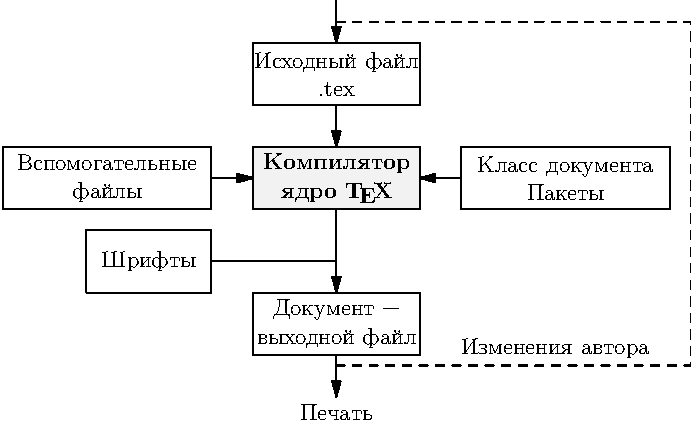
\includegraphics[scale=0.8]{CH-MainFile/Fig-MainFile-1}
\caption{Упрощённая схема работы}
\label{Fig:MainFile-1}
\end{figure}

В процессе работы компилятора в зависимости от задач \TeX\ создаёт \bi{вспомогательные файлы}\index{Файл!вспомогательный}, которые необходимы, например, для хранения данных о ссылках или записи информации о компиляции. Среди них можно выделить следующие основные типы файлов по их расширению:
% % ССЫЛКИ - 4 слова в одном предложении
\begin{description}
\item[\texttt{aux}] отвечает за перекрёстные ссылки и содержит информацию о настройках языка и о тех объектах, на которые можно ссылаться (более подробно см.\ главы~\ref{CH:Sections}, \ref{CH:Itemize}, \ref{CH:Lists}, \ref{Floats});
\item[\texttt{toc}] отвечает за создание оглавления и содержит данные о всех заголовках и страницах, где они начинаются (подробнее см.\ главу~\ref{CH:Sections});
\item[\texttt{lof}, \texttt{lot}] отвечают за списки рисунков и таблиц (см.\ главу~\ref{CH:Floats});
\item[\texttt{log}] содержит информацию о ходе компиляции и возможных предупреждениях и ошибках. Обычно эта информация выводится в специальном окне редактора;
\item[\texttt{idx}, \texttt{ilg}, \texttt{ind}] отвечает за предметные указатели (подробнее в гл.~\ref{CH:Lists});
\item[\texttt{bbl}] появляется при создании списка литературы с помощью Bib\TeX\ (см.\ главу~\ref{CH:BibTeX}).
\end{description}

Исходный файл, в котором происходит вся работа автора, имеет чёткую структуру и состоит из двух основных частей: \emph{преамбулы} и \emph{основного текста}.

\index{Преамбула}\bi{Преамбулой} называется та часть исходного файла, в которой вводятся все необходимые определения и настройки, такие как \emph{класс документа}, \textit{пакеты}, параметры и \textit{макроопределения}. Преамбула основного файла всегда начинается с определения \emph{класса документа}.

\begin{note}
В преамбуле может быть сколько угодно пустых строк, которые никак не влияют на результат.
\end{note}

\index{Текст!основной}\bi{Основной текст} "--- это непосредственно та часть исходного файла, в которой автор набирает всё то, что он хочет видеть в своем документе: текст, таблицы, рисунки и~т.~д. По сути здесь находится весь текст с включёнными в него командами, которые непосредственно влияют на текст, его форматирование и внешний вид.

Таким образом, структуру основного файла можно представить в следующем виде:
\begin{verbatim}
Начало исходного файла
  Преамбула:
   определения и настройки

  Основной текст:
   смысловая часть текста и включённые в неё команды
Конец исходного файла
\end{verbatim}

\begin{note}
Важно отметить, что исходный файл не должен содержать какие бы то ни было выделения цветом, шрифтовые выделения, разбивку на страницы и другие <<художественные>> элементы. Компилятор должен получить <<чистый>> текстовый файл, поэтому наиболее простыми вариантами для набора будут специальные \TeX-редакторы (см.\ параграф~\ref{Sec:Editors}).
\end{note}





% % ========================================================================
\section{Синтаксис и команды языка}\label{Sec:Syntaxis}

Для дальнейшего и более детального изучения строения исходного файла и его содержания рассмотрим вначале особенности синтаксиса\index{Синтаксис языка \TeX} языка системы \TeX\ и языка макроопределений \LaTeX.

% Садовский П.А., 2005/09/18 \bi{Язык системы \TeX}\index{Язык \TeX} и его последующее развитие (например, макропакет \LaTeX\ на основе языка \TeX) не является просто языком разметки, с помощью которого в процессе трансляции документ форматируется определённым образом. Это, можно сказать, полноценный и очень мощный язык программирования, включающий в себя различные средства (например, операторы логических переходов, переопределения команд и~пр.). % Садовский П.А., 2005/09/18

В тексте исходного файла можно использовать латинские и русские буквы \texttt{A}... \texttt{Z}, \texttt{a}... \texttt{z}, \texttt{А}... \texttt{Я}, \texttt{а}... \texttt{я}, цифры \texttt{0}... \texttt{9}, символы:

\begin{verbatim}
. , : ; ! ? ( ) [ ] ' ` - * /  @ | < > + = " №
\end{verbatim}
Кроме того, существует десять зарезервированных символов:
\begin{verbatim}
\ { } $ & # % ^ _ ~
\end{verbatim}
Их употребление в тексте может привести к ошибке или нежелательным последствиям "--- в большинстве случаев, если даже и не будет ошибки, результат вряд ли совпадёт с ожидаемым. Более подробно набор таких символов описан в последующих главах (например, см.\ параграф~\ref{Sec:Znaki}).

\begin{note}
Отметим, что символы <<\verb"|">>, <<\verb|<|>> и <<\verb|>|>> могут встречаться и в командах, но их использование в обычном тексте не приведёт к~ошибке, правда, результат может быть неожиданным.
\end{note}

Команды и макроопределения, составляющие разметочную часть языка \TeX, имеют ряд особенностей и~легко отличаются от обычного текста. %Для их написания используются наиболее редкие для повседневных документов символы.

\bi{Команда}\index{Команда \TeX} "--- это последовательность символов, которая воспринимается транслятором не как обычный текст, а~как указание для совершения какого-либо действия над документом или его частью.

Одной из самых простых команд системы \TeX\ является одиночный символ \verb|%|. Если поставить такой символ в тексте, то все, что идёт после этого символа до перехода на новую строку будет рассматриваться как комментарий и не будет восприниматься компилятором.

Команда системы \TeX{} "--- это либо символы \verb|{|, \verb|}|, \verb|$|, \verb|%|, \verb|&|, либо последовательность символов, которая начинается с <<обратной косой черты>> \verb|\|, например, \verb|\newpage|, \verb|\usepackage[T2A]{fontenc}| и~т.~д., в общем случае имеет вид:
\begin{verbatim}
\<название>[<параметры>]{<параметры>}...{<параметры>}
\end{verbatim}
Заметим, что символ <<\verb|\|>> и \verb|<название команды>| не разделяются пробелом. Окончанием команды является ближайший идущий после неё пробел, переход на новую строку или любой символ, не являющийся командой или буквой латинского алфавита. В квадратных скобках указываются необязательные параметры, а в фигурных "--- обязательные.

В случае, если необязательные \texttt{<параметры>} отсутствуют,  пустые квадратные скобки как ставить, так и опускать их. Например, следующие две команды эквивалентны:
\begin{verbatim}
\<название>[]{<параметры>}
\<название>{<параметры>}
\end{verbatim}

\begin{note}
Во всех описаниях начало и конец строки-названия отмечены открывающей и закрывающей угловыми скобками \verb|<| и \verb|>| соответственно. Они не являются частью команды и введены только для обозначения символьных последовательностей (имён) как единого целого.
\end{note}

Пара символов \verb|{| и \verb|}| используется как ограничители групп текста, которые входят в состав сложных команд или над которым производится некоторое действие. Символ \verb|$| иногда может встречаться в сложных командах, а также (как и символы \verb|_| и \verb|^|) он может использоваться при наборе математических формул.

Отдельно следует выделить команды, которые идут парой и модифицируют текст, заключённый между ними.

\bi{Окружением}\index{Окружение} будем называть <<сдвоенную>> команду системы \LaTeX, выполняющую определённые операции над текстом, заключённым в <<тело окружения>>. Обычно эта команда имеет вид:
\begin{verbatim}
\begin{<имя окружения>}[<параметры>]
  <Тело окружения>
\end{<имя окружения>}
\end{verbatim}

Параметр \verb|<имя окружения>| является обязательным и представляет собой строку "--- название окружения. Дополнительные \texttt{<параметры>} зависят от конкретного окружения и будут каждый раз оговариваться отдельно.

Под \verb|<телом окружения>| будем понимать ту часть текста, к которой применяется данное окружение, т.~е. текст, заключённый между командами начала \verb|\begin{<имя окружения>}| и окончания \verb|\end{<имя окружения>}|.

Окружения в системе \LaTeX\ играют очень важную роль, а их количество и разнообразие очень сильно упрощает работу над текстом и вёрстку документа. Следует отметить, что каждому началу окружения \verb|begin| всегда должен соответствовать свой \verb|end| с тем же самым именем, иначе компилятор выдаст сообщение об ошибке.

\begin{note}
Любая последовательность символов, идущая после \verb|%| до ближайшего перехода на новую строку, рассматривается как комментарий и не воспринимается компилятором.
\end{note}





% % ========================================================================
\section{Простейший вид исходного файла. Первый документ}\label{Sec:FirstDoc}

Как упоминалось ранее, исходный файл, в котором происходит вся работа, состоит из \emph{преамбулы} и \emph{основного текста}. Преамбула всегда начинается с определения класса документа. \bi{Стиль документа}\index{Документ!стиль} или \bi{класс документа}\index{Документ!класс} "--- это тип того документа, который создаёт автор. От выбора этого типа зависят исходные размеры листа и текстовых полей, оформление заголовков, автоматическая нумерация и многие другие настройки.

Класс документа задаётся командой
\begin{verbatim}
\documentclass{<класс документа>}
\end{verbatim}
где обязательный параметр \verb|<класс документа>| представляет собой название того класса, который будет использоваться при создании документа и которому соответствует одноимённый файл
\begin{verbatim}
<класс документа>.cls
\end{verbatim}
При компиляции \TeX\ ищет файл соответствующего класса \verb|*.cls| и берёт из него основные определения и параметры. 

Основной текст, в котором заключена вся смысловая часть документа, набирается в окружении \texttt{document}, т.~е.
\begin{verbatim}
\begin{document}
   <основной текст>
\end{document}
\end{verbatim}

\begin{note}
Любой текст, идущий после строки \texttt{\textbackslash end\{document\}}, не воспринимается \TeX'ом и выводиться не будет.
\end{note}

Таким образом, минимально необходимый для начала работы исходный файл можно представить следующим образом:
\begin{verbatim}
\documentclass{<класс документа>}

\begin{document}
   <основной текст>
\end{document}
\end{verbatim}

Выведем на листе надпись ``This is \TeX!'' с характерным написанием названия \TeX\indcom{TeX}, которое задаётся командой \verb|\TeX|. Эта надпись пока что будет на английском, поскольку этот язык поддерживается по умолчанию.
\begin{example}
This is \TeX!
\end{example}
\begin{release}
\begin{verbatim}
\documentclass{article}

\begin{document}
This is \TeX!
\end{document}
\end{verbatim}
\end{release}

После набора этого текста в \TeX-редакторе и его последующей компиляции в любой из форматов вывода, например, в \verb|pdf|, получаем следующий результат: на листе формата А4 вверху будет нужная нам фраза, а внизу "--- номер страницы.

\begin{remark}
Мы использовали в этом примере один из стандартных классов \texttt{article} (статья), общее описание которого, а также других классов, приводится в параграфе~\ref{Sec:StandardClasses}.
\end{remark}

Сделаем краткие выводы, необходимые для работы.

\begin{enumerate}
\item Исходный файл всегда начинается командой \texttt{\textbackslash documentclass} с указанием класса документа.
\item Основной текст набирается строго внутри окружения \texttt{document}.
\item Любой текст, идущий после строки \texttt{\textbackslash end\{document\}}, не воспринимается \TeX'ом и выводиться не будет.
\item Между определением класса документа и основным  текстом, т.~е.\ в преамбуле, могут идти различные настройки и дополнительные определения.
\end{enumerate}

\begin{note}
Здесь и далее мы будем говорить, что если нужно что-то определить или добавить в преамбулу, это означает, что необходимые строки добавляются \emph{после} определения класса документа и \emph{до} начала окружения \texttt{document}.
\end{note}







% % ========================================================================
\section{Подключение русского языка}\label{Sec:Russian}

В предыдущем примере мы выводили на экран фразу на английском языке. Для использования русского языка нам нужно будет использовать дополнительные \emph{пакеты}.

\bi{Пакет} (или package)\index{Пакет}\index{Package} "--- это набор макрокоманд или макроопределений, расширяющих возможности системы. Эти команды оформлены в виде отдельного одноимённого файла \verb|<пакет>.sty|, где последовательность \verb|<пакет>| "--- имя соответствующего пакета. Более подробно макрокоманды описываются в главе~\ref{CH:Macros}.

Для того чтобы загрузить пакеты с дополнительными макроопределениями для расширения функциональных возможностей системы, используется команда \indcmd{usepackage}, которая имеет вид:
\begin{verbatim}
\usepackage[<опции>]{<пакет>}
\end{verbatim}
Эта команда имеет два параметра. Необязательные \texttt{<опции>} определяют особенности подгружаемого пакета (или пакетов) и могут быть опущены. В этом случае можно как ставить пустые квадратные скобки, так и опускать их. Например, следующие две команды эквивалентны:
\begin{verbatim}
\usepackage[]{<пакет>}
\usepackage{<пакет>}
\end{verbatim}
Параметр \verb|<пакет>| определяет непосредственно сам пакет (точнее, его имя), воплощённый в одноимённом файле под названием \verb|<пакет>.sty|. Заметим также, что эта команда допускает перечисление нескольких пакетов, имена которых указываются через запятые, например,
\begin{verbatim}
\usepackage{<пакет1>,<пакет2>,...,<пакетN>}
\end{verbatim}

\begin{note}
Если были указаны какие-либо параметры, то они передаются \emph{всем} пакетам, указанным в аргументе \comm{usepackage}. Так как этими пакетами могут поддерживаться не все параметры, то следует быть осторожным.
\end{note}

Для использования русского языка необходимо в преамбуле добавить следующие строки
\begin{verbatim}
\usepackage[cp1251]{inputenc}
\usepackage[T2A]{fontenc}
\usepackage[russian]{babel}
\end{verbatim}

Первая команда загружает пакет \texttt{inputenc}, который определяет, какую входную кодировку должен использовать \LaTeX\index{Файл!кодировка}\index{Пакет!inputenc} (см.\ параграф~\ref{CH:Text}).

Вторая команда загружает пакет \texttt{fontenc}, определяющий кодировку шрифта\index{Пакет!fontenc}. В данном случае загружается кодировка \texttt{T2A}, которая используется при русскоязычном наборе. Кодировка шрифта для набора латинского шрифта (английского языка) загружается по умолчанию.

Третья команда загружает пакет, позволяющий использовать и вводить русский язык, корректно расставлять русские переносы\index{Пакет!babel}. Именно поэтому в качестве необязательного параметра указан \texttt{russian}. Для подключения других языков и их переключения в процессе работы "--- см.\ главу~\ref{CH:Fonts}.\medskip

Пусть нам нужно вывести на экран (или последующую печать) следующую строку:
\begin{verbatim}
В любой работе есть место творчеству.
\end{verbatim}

В исходном файле необходимо написать следующее:
\begin{verbatim}
\documentclass{article}
\usepackage[cp1251]{inputenc}
\usepackage[T2A]{fontenc}
\usepackage[russian]{babel}

\begin{document}
В любой работе есть место творчеству.
\end{document}
\end{verbatim}

После компиляции в любой из форматов вывода, на выходе получается следующий результат (при просмотре в программе, соответствующей формату выходного файла): на листе формата А4 внизу будет стоять номер~1, а вверху страницы будет выведена надпись:
\medskip

В любой работе есть место творчеству.

\medskip

Таким образом, приведённый пример уже позволяет работать в системе и набирать тексты на русском языке. Дальнейшие главы будут посвящены тому, как лучше набирать и оформлять тот или иной элемент документа.


\endinput
%Команда {documentclass}\index{Документ!класс}
%\begin{verbatim}
%\documentclass[<параметры класса>]{<класс документа>}
%\end{verbatim}
%имеет два параметра.
%
%Заключённые в квадратные скобки \verb|<параметры класса>| оп\-ределяют размеры листа, шрифта, режима вывода текста и~т.~д. Квадратные скобки указывают на то, что этот параметр является \textit{необязательным}, следовательно, если его опустить (и опустить сами скобки), то все настройки будут ставиться <<по умолчанию>>, например,
%\begin{verbatim}
%\documentclass{<класс документа>}
%\end{verbatim}
%Параметр \verb|<класс документа>|, заключённый в фигурные скобки, является строго обязательным и представляет собой название класса, которому соответствует одноимённый файл
%\begin{verbatim}
%<класс документа>.cls
%\end{verbatim}
%При начале трансляции файл соответствующего класса \verb|*.cls| сначала ищется в текущей папке, в которой лежит исходный файл, а затем, при его отсутствии, в корневых каталогах \TeX'а, указанных в программе <<Mik\TeX{} Options>> на вкладке <<Roots>>, в том порядке, в котором они указаны (обычно это каталоги \texttt{localtexmf} и \texttt{texmf}).

%Поэтому, при создании своих классов или использовании не\-стандартных, соответствующий файл класса с расширением \verb|cls| проще всего, да и лучше, поместить в папку, где находится исходный файл.

%Под определениями и настройками подразумеваются любые настройки документа: поля, шрифты и многое--многое другое. Все они должны находиться после определения класса и до начала основного текста. \bi{Пакет}\index{Пакет}\index{Package} "--- это набор макрокоманд или макроопределений, расширяющих возможности системы и оформленных в виде отдельного <<стилевого>> файла \verb|<пакет>.sty|, где последовательность \verb|<пакет>| "--- имя соответствующего пакета.







	% Заморожено: 12 Января 2013
	
% % ==== Параграф ==========================================================
	\section{Стандартные классы}\label{Sec:StandardClasses}

В предыдущих примерах мы использовали один из стандартных классов, которые предопределены в системе \LaTeX. Эти классы были изначально созданы на основе американских стандартов и общепринятых правил и, поэтому, часто не самым лучшим образом подходят под отечественные реалии. Тем не менее, использование стандартного класса для абсолютного большинства пользователей является необходимым, поскольку написание своего класса процесс очень сложный и абсолютно бессмысленный, если, например, нужно сделать какую-то учебную работу. 

Поэтому мы рассмотрим основные стандартные классы, которые описаны в системе \LaTeX, а в последующих главах будем учиться их настраивать. 

Класс \texttt{article}\index{article}\index{Документ!класс!article} "--- статья "--- лучше всего подходит для набора небольших статей, курсовых работ и проектов, заметок, докладов и~т.~п. В этом классе по умолчанию установлен односторонний набор (поэтому поля на всех страницах одинаковы), сквозная нумерация всех нумеруемых объектов (сносок, формул, таблиц, рисунков). Наверно, в большинстве случаев это наиболее приемлемый класс, поэтому именно он рекомендуется в студенческих работах.

Класс \texttt{report}\index{report}\index{Документ!класс!report} "--- отчёт "--- предназначен для набора отчётов по научной и исследовательской работе. Этот класс поддерживает по умолчанию двусторонний набор, но ещё не дотягивает до того, чтобы набирать книги без сложных предварительных настроек.

Класс \texttt{book}\index{book}\index{Документ!класс!book} "--- книга "--- в большинстве случаев используется для создания брошюр и книг. При использовании этого класса документ будет оформлен как книга: двусторонняя разметка страницы (учитываются правые и левые поля, нумерация страниц), колонтитулы, особенности оформления рубрик (например, главы автоматически начинаются с новой нечётной страницы) и многое другое.

Каждый класс имеет ряд определённых особенностей, которые были заложены при их создании, например, глубину вложения и оформление разделов, их нумерацию, оформление титульных листов, оглавлений и многое другое. Однако эти классы построены по одной схеме, да и отличие состоит не в каких-то ключевых моментах, а скорее в некоторых частностях. Тем не менее создание классов представляет собой сложный и очень трудоёмкий процесс, впрочем, как и их видоизменение. Приведённые выше основные классы документа имеют свои возможные \verb|<параметры класса>|, которые более подробно рассмотрены в приложениях в конце книги (стр.~\pageref{struct::ClassOptions->Appendix}). Некоторые из этих свойств будут вводиться по ходу изложения.


\endinput
 		%\section{Стандартные классы}
%	% Писать - Петя
%	\section{Форматы ввода и вывода}
%	
% % ==== Подпараграф =======================================================
	\subsection{Форматы ввода}\label{Sec:InFormats}


\endinput
 				%\section{Форматы ввода} % cp1251, cp1251-light,
%													%utf8 - Петя (под вопросом)
	
% % ==== Подпараграф =======================================================
	\section{Форматы вывода}\label{Sec:OutFormats}

Система \TeX\ может переводить текст в формат DVI (Device Independent), PDF (Portable Document Format) и PS (PostScript). Все эти форматы являются плат\-фор\-мно-независимыми, однако каждый из них имеет свои особенности, которые зачастую предопределяют их использование.

\textbf{Формат DVI}\index{Формат вывода!DVI} очень хорошо подходит для предварительного просмотра текста в процессе набора, вёрстки и пробной печати. Однако, хотя он и называется <<device independent>> и одинаково хорошо приспособлен для вывода на печать или экран, при переносе с одной системы на другую может некорректно отображаться, поскольку зависит от настроек программной среды: наличия шрифтов, вспомогательных средств и~пр.

\textbf{Язык PostScript}\index{Формат вывода!PostScript}, базирующийся на языке Forth, является одним из плат\-фор\-мно-не\-за\-ви\-си\-мых языков описания страниц и использует векторную форму описания. При этом подразумевается, что устройство (будь то дисплей, принтер, плоттер) самостоятельно выполняет преобразование векторного представления в растровое с учётом своей разрешающей способности.

Для каждого из устройств результирующее растровое изображение будет различным, однако размеры, положение, координаты вершин объектов и прочие геометрические параметры обязаны совпадать. Компания Adobe обладает лицензией на все реализации  PostScript, что, с одной стороны, значительно влияет на цену устройств, поддерживающих этот язык, а с другой "--- обеспечивает почти полную совместимость с любой компьютерной платформой. Чрезвычайно широкое распространение PostScript нашел на платформе Apple Macintosh.

Язык имеет средства описания прямых линий, углов, прямоугольников и кривых третьего порядка, возможность отображения линий любой толщины и любого цвета (цвет может быть представлен в моделях Pseudo-Greyscale, RGB и CMYK). Текст полностью интегрирован с графикой, а текстовые символы, как предопределённые, так и пользовательские, могут быть объектами любого графического оператора.

PostScript позволяет описывать растровые изображения любого разрешения с использованием различных цветовых моделей. Общая система координат поддерживает комбинации следующих преобразований: масштабирование, поворот, зеркальное отображение. Преобразования применяются одновременно ко всем элементам страницы, включая текст, графические примитивы и растровые изображения.

Вторая версия "--- PostScript Level 2 (старое название Sup\-ra) "--- обеспечила, кроме того, платформно-независимое отображение цвета, сжатие данных и улучшенные алгоритмы преобразования полутоновых изображений.

В последней реализации "--- Adobe PostScript~3 "--- ядро интерпретатора претерпело значительные изменения, по сравнению с предыдущей версией увеличилась производительность.

Encapsulated PostScript был создан для обеспечения межплатформенной переносимости рисунков в формате PostScript. Основное отличие EPS заключается в том, что возможности формата ограничиваются описанием одной страницы. Объекты страницы EPS не влияют на изображения, находящиеся за пределами этой страницы. Файл EPS может содержать растровый эскиз изображения для предварительного просмотра (чаще всего в формате TIFF).

Для просмотра файлов PS (EPS) необходима программа-интерпретатор языка PostScript, например GhostScript и программа просмотра GSView, или редакторы, воспринимающие данный формат "--- Adobe Illustrator, Corel Draw, Adobe Acrobat. В числе прочих данный формат воспринимает и Adobe Acrobat Reader.

\index{Формат вывода!PDF}\textbf{Формат PDF} был создан компанией Adobe как универсальный формат для хранения и переноса данных на разных вычислительных платформах. Файлы формата PDF <<весят>> больше, чем файлы DVI, но основным их преимуществом является <<истинная>> платформенная независимость (проблема с наличием шрифтов решается путём интегрирования использованных символов шрифта в документ, что положительно сказывается на внешнем виде и отрицательно "--- на объёме) и неизменность при печати. Являясь по сути графическим объектом, этот формат прекрасно отображает графику (рисунки многих форматов, от JPEG до EPS), поддерживает <<художественное>> оформление текста и создание презентаций с гиперссылками.

В отличие от формата DVI, в файл формата PS, EPS или PDF можно внедрить символы используемых шрифтов (или, в случае PS/EPS "--- сохранить символы как кривые), что позволяет на \textit{любом} компьютере или печатающем устройстве увидеть в точности такой результат, какой необходим "--- даже если соответствующая гарнитура отсутствует.



\endinput
 				%\section{Форматы вывода} %




% % ==== ЧАСТЬ =========================================================
% % ==== Простой текст =================================================
	\part{Простой текст}


% % ==== Набор простого текста =========================================
	% Заморожено: 12 Января 2013
	\input{CH-Text/Sec-Text}


% % ==== Шрифты и их внешний вид =======================================
	% Вычитывать: 13 Ноября 2012
	\input{CH-Fonts/Sec-Fonts}


% % ==== Разметка текста и страницы ====================================
	% Вычитывать: 23 Июля 2013
	\input{CH-Layout/Sec-Layout}
%	\input{CH-Layout/Example-Layout} %\section{Продолжение примера}


% % ==== Секционирование и рубрикация ==================================
	% Проверять: 23 Июля 2013
	\input{CH-Sections/Sec-Sections}
%	\input{CH-Sections/Example-Sections} %\section{Продолжение сквозного примера}


% % ==== Другие элементы оформления ====================================
	% Дописывать: 13 Ноября 2012
	\input{CH-GeneralDesign/Sec-GeneralDesign} %
%	\input{CH-GeneralDesign/Example-GeneralDesign}


% % ==== Списки и перечисления =========================================
	% Добавить примеры и вычитывать: 23 ноября 2012
	\input{CH-GeneralDesign/Sec-Itemize} %


% % ==== Предметные и авторские указатели ==============================
% % ==== Списки обозначений, Глоссарии =================================
	% Дописывать много всего: 23 ноября 2012
	\input{CH-Lists/Sec-Lists} %
	% Предметный указатель, более подробно


% % ==== Библиографическое описание ====================================
	% Пишут все
	% Нужно делать, в основном про BibTeX
	\input{CH-BibTeX/CH-BibTeX} %\chapter{Библиографическое описание}\label{CH:BibTeX}
	% Не знаю, кто будет писать...
	% Включить сюда создание списка лит-ры - обычного, а также БибТеХ
	%\section{Продолжение сквозного примера}
	% Описание по ГОСТ...



% % Название <<формулы>> - подумать над переделкой
% % ==== ЧАСТЬ =========================================================
% % ==== Формулы =======================================================
	\part{Формулы}\label{Part:Math}


% % ==== Основы математики =============================================
	% Вычитывать: 8 Августа 2013
	\include{CH-Math/Math-Basic}


% % ==== Тонкости математики ===========================================
	% Вычитывать: 8 Августа 2013
	\include{CH-Math/Math-Advance}


%% % Выравнивание формул типа align, но чтобы там можно было набирать в том числе и многострочные ф-лы.
%% % пакет KUVIO для рисования диаграмм. Наверно, надо посмотреть его.
%% % \mathindent, более детально про нумерацию и выравнивание формул, особенно многострочных

% % ДОБАВЛЕНИЯ


% % ==== Химические формулы ============================================
	% Вычитывать: 13 Ноября 2012
	\input{CH-Chemistry/Chemistry}
	% Договорились, что структурные формулы не нужны.


% Информатика: листинги программ и пр.
%\chapter{Физика и Биология}
%
%% Виталик - физическое и Биологическое
%% Правда, вопрос - а что конкретно сюда совать?
%% Можно что-то типа схем, рисунков + формулы. Физические задачки и т.п.
%% (очень неплохо сделаны примеры в мануале Tikz - можно по аналогии)
%% Сюда же можно добавить что-то типа  Системотехники...

% % Как вариант - добавить примеры оформления геометрических и всяких там задачек механики - учитывая опыт пакета TIKZ из предыдущих глав - получится вполне себе интересная глава (механика, геометрия, всякие там схемы электротехники и пр. - можно набрать кучу примеров)






% % ==== ЧАСТЬ =========================================================
% % ==== Графические объекты ===========================================
	\part{Графические объекты: таблицы и рисунки}


% % ==== Плавающие объекты =============================================
	% Вычитывать: 9 августа 2013
	\include{CH-Floats/Floats}

% % ==== Таблицы =======================================================
	% Вычитывать: 9 августа 2013
	\include{CH-Tables/Tables}

% % ==== Многостраничные таблицы =======================================
	% Вычитывать: 9 августа 2013
	\include{CH-Tables/MTables}

% % ==== Рисунки =======================================================
	% Вычитывать: 9 августа 2013
	\include{CH-Figures/Figures}
	% Дать ссылку на пакет TIKZ


%%% % ==== Пакет TikZ ====================================================
%%		% По сути - пусто... нужно много писать!
%%		% Тикз - пишут все!!!
%%		\include{CH-Tikz/TikZPkg}  % ???
%%		\section{Продолжение сквозного примера}


%%% % ==== Asymptote =====================================================
% % %\include{CH-Asymptote/AsymptotPkg}			
%% 		% Оставить только для рисования графиков...




% % ==== ЧАСТЬ =========================================================
% % ==== Программирование в ТеХ ========================================
	\part{Программирование в ТеХ}\label{Part:Programming}



% % ==== Макрокоманды ==================================================
	\include{CH-Macros/Macros}
%	\section{\textcolor{blue}{Стилевые файлы}}
%		\subsection{\textcolor{blue}{Структура стилевого файла}}
%		\subsection{\textcolor{blue}{Изменение стандартных элементов оформления}}
%		\subsection{\textcolor{blue}{Создание новых типов разделов}}
%		\subsection{\textcolor{blue}{Продолжение № 10 сквозного примера}}


%Fragile and Robust commands
%LaTeX commands are either robust or fragile. Fragile commands need special care if they are part of a moving argument.
%
%Arguments to some LaTeX commands are called moving arguments because they may be "moved" to other places in the document. For example, the argument of Sectioning comands may be moved to the Table of Contents. Other examples of moving arguments include:
%
%	arguments of \caption commands
%	terminal input and output, \typeout and \typein
%	commands that produce page headings
%	the Letter Environment
%	the \thanks command
%	an @ expression in the Array or Tabular environment
%
%A fragile command that appears in a moving argument must be preceded by a \protect command. The \protect applies only to the immediately following command; if arguments of this command also contain fragile commands, the latter must be protected with their own \protect.


% % Можно взять у Марчевского некое подобие стилевика, его использовать в качестве примера
% % Отедельно дать про набор статей!
% % Списки литературы, римские цифры



%%% % ==== ЧАСТЬ =========================================================
%%% % ==== Особенности оформления электронных документов =================
%%	\part{Особенности оформления электронных документов}
%%
%%	\input{CH-Electronic/Sec-Electronic}
%%	
%%	\chapter{Презентации}
%%		\section{Стандартные пакеты}
%%		\section{Типы слайдов}
%%		\section{Дополнительные возможности}
%%%				% В качестве пожелания: добавить гиперссылки на внешние файлы (например, видео),
%%% 				% т.к. обычное видео туда сунуть нельзя.
%%%				% Дать сюда гиперссылки (ВСЕ), убрать их из Секционирования
%%%				% пакеты hyperref или url
%%		\section{Пример}




%% % ==== ЧАСТЬ =========================================================
%% % ==== Дополнения ====================================================
%		% Основы набора нот
%		\input{Addons/Notes}

%		% Шахматные партии
%		%\input{Addons/Chess}

% Кроссворды, судоку...





%% % ==== ЧАСТЬ =========================================================
%% % ==== Приложения ====================================================
%	\part{Приложения}
%%	\addcontentsline{toc}{part}{Приложения}
%
%
%	% \chapter{Наиболее частые пакеты и их описание}
%		\input{Appendix/App-Symbols} %
%%	%	\input{Appendix/Packages} %


% % Возможно имеет смысл дать краткое описание пакетов и перечислить все команды, которые мы использовали из этих пакетов - чтобы была возможность найти необходимый пакет для подключения. В тексте не всегда быстро можно найти. Либо учесть это каким-либо образом в предметном указателе.
% ДАТЬ ССЫЛКИ НА СТРАНИЦЫ
%% Например:
%% \verb|package 1| --- описание пакета (кратенько)
%%    \команда 1             \команда (n-1)
%%    \команда 2             \команда n
%%
%% \verb|package 2| --- описание пакета (кратенько)
%%    \команда 1             \команда n
%%    \команда 2
%% Ну или давать в 3 столбца --- тут уже дело вкуса.




% % Как вариант: давать в предметном указателе (только для команд, которым нужно подключение пакета):
% %		Команда (пакет), стр.
% % Хотя, конечно, это сильно загрузит указатель.
% % Можно еще давать так:
% %		Команда, стр. (где встречается в тексте), стр. (где она в списке пакетов, например, курсивом)

	\backmatter



% % ==== ГЛАВА =========================================================
% % ==== Предметный указатель ==========================================
	\addcontentsline{toc}{chapter}{\indexname}
	{\normalbaselines\footnotesize\printindex}



% ФУНКЦИОНАЛЬНЫЙ УКАЗАТЕЛЬ




% % ==== ГЛАВА =========================================================
% % ==== Список литературы =============================================
	\input{References/References} %

%%% % A.~Syropoulos, A.~Tsolomitis, N.~Sofroniou, Digital typography using LaTeX. Springer.

\clearpage
\thispagestyle{empty}
\mbox{}\vfill

\begin{quote}\em
Только кончая задуманное сочинение, мы уясняем себе, с чего нам следовало его начать.\\[.3cm]
\mbox{}\hspace{\fill}\rm Блэз Паскаль
\end{quote}


\end{document}
